\section{Pedestrian Dead Reckoning} \label{sec:IMUPositioning_eval}
This section describes the evaluation of the \gls{pdr} algorithm using Madgwick orientation filter and Extended Kalman Filter for heading estimation.

%We will present a cumulative distribution graph of the evaluation results of the two experiments, one for each heading estimation filter. 
%Furthermore, 
An average positioning error has been computed of all positioning errors, but it is important to note that this value is highly affected by the length of each path in the evaluation. This is because the positioning error is accumulative for \gls{pdr}, as mentioned in \textbf{\autoref{sec:IMUPositioning}}. Therefore, the shorter a path in the evaluation is, the more the average positioning error is dragged towards a lower value, and therefore, this value does not truly represent the performance of a \gls{pdr} implementation of one heading estimation filter. However, the average positioning error can be used to compare the different \gls{pdr} implementations with the two different heading estimation filters, since both are evaluated on the same data and paths. Furthermore, the position errors of both filters for selected paths have been shown and evaluated on, as seen in \textbf{\autoref{PDR:results}}. The most remarkable diagrams are the diagrams shown in \textbf{\autoref{fig:pdr_performance}}. As it can be seen from the experiment results in \textbf{\autoref{PDR:results}}, the \gls{pdr} algorithm using Madgwick Filter for heading estimations performs best, since its positioning error is lower than the \gls{pdr} algorithm using Extended Kalman Filter for heading estimation. Furthermore, as explained in \textbf{\autoref{sec:IMUPositioning}}, the \gls{pdr} algorithm drifts the longer the path is, resulting in higher positioning errors per measurement. It is noticeable that the \gls{pdr} algorithm improves its estimations per measurement in \textbf{\autoref{fig:pdr_performance}(c)}. The reason for this might be that the \gls{pdr} algorithm makes three wrong heading estimations at measurement 748, 1654 and 2089 that turns the pedestrian toward the ground truth path.

The mean positioning errors across all paths for Madgwick and Extended Kalman Filter are 34.78 meters and 43.83 meters, respectively.

\begin{figure}[H]
\centering
\SetFigLayout{2}{2}
  \subfigure[]{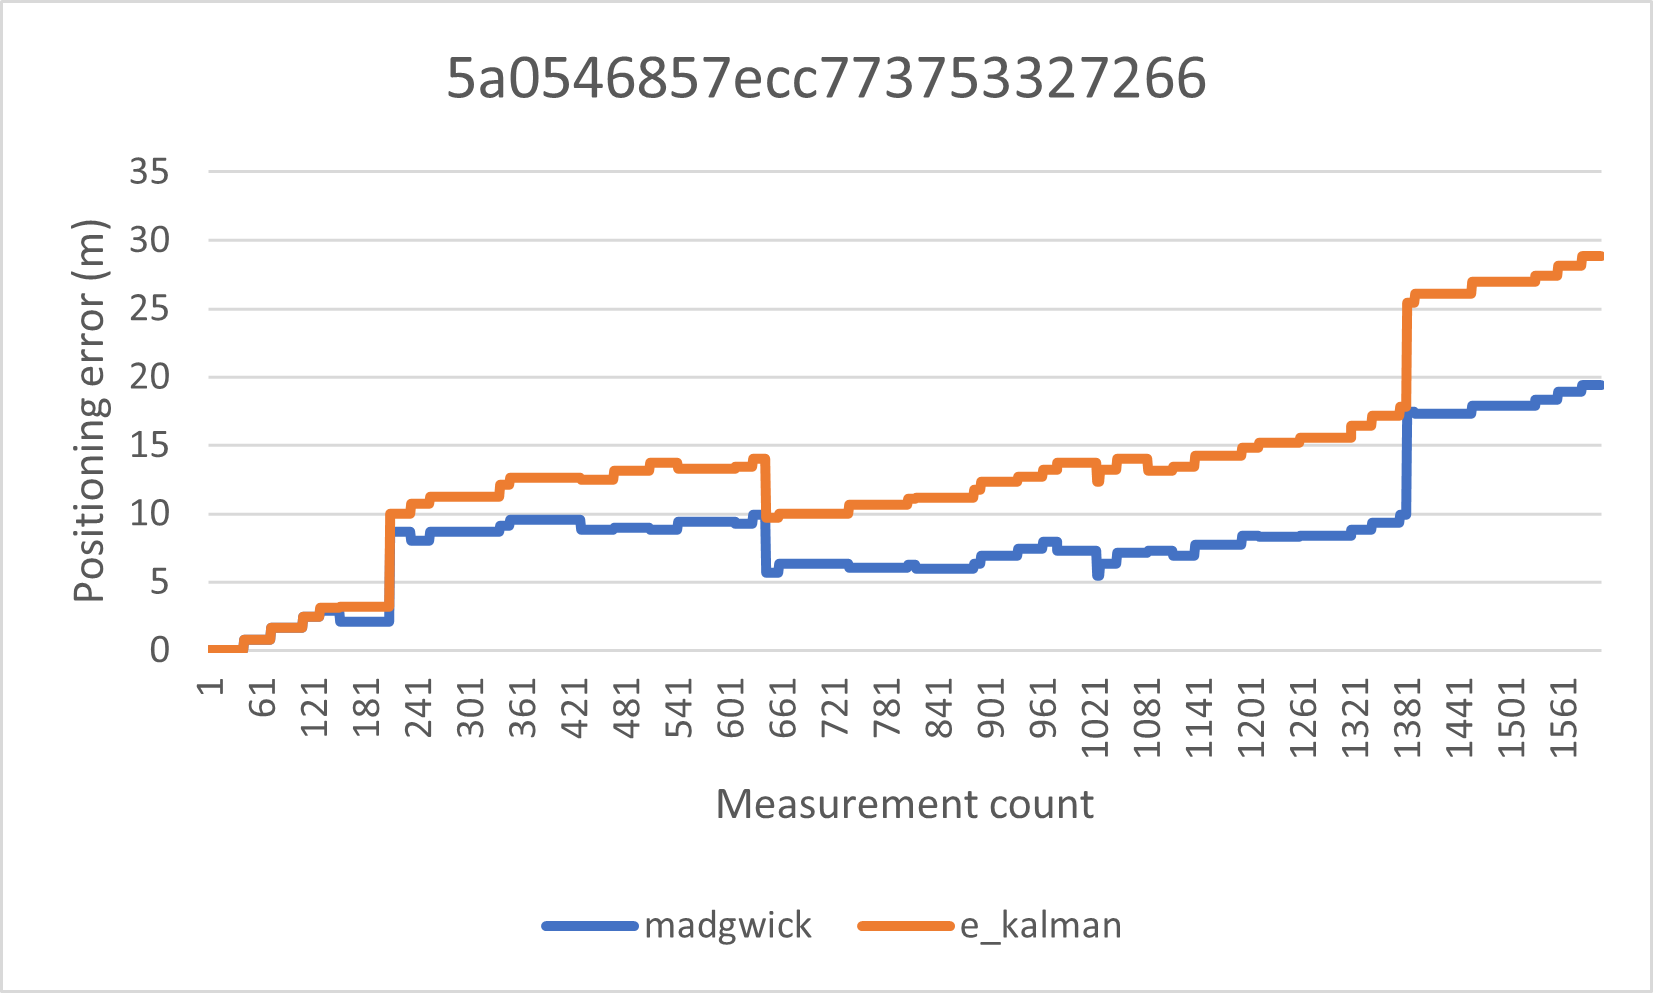
\includegraphics{Images/Experiments/pdr/pdr1.png}}
  \hfill
  \subfigure[]{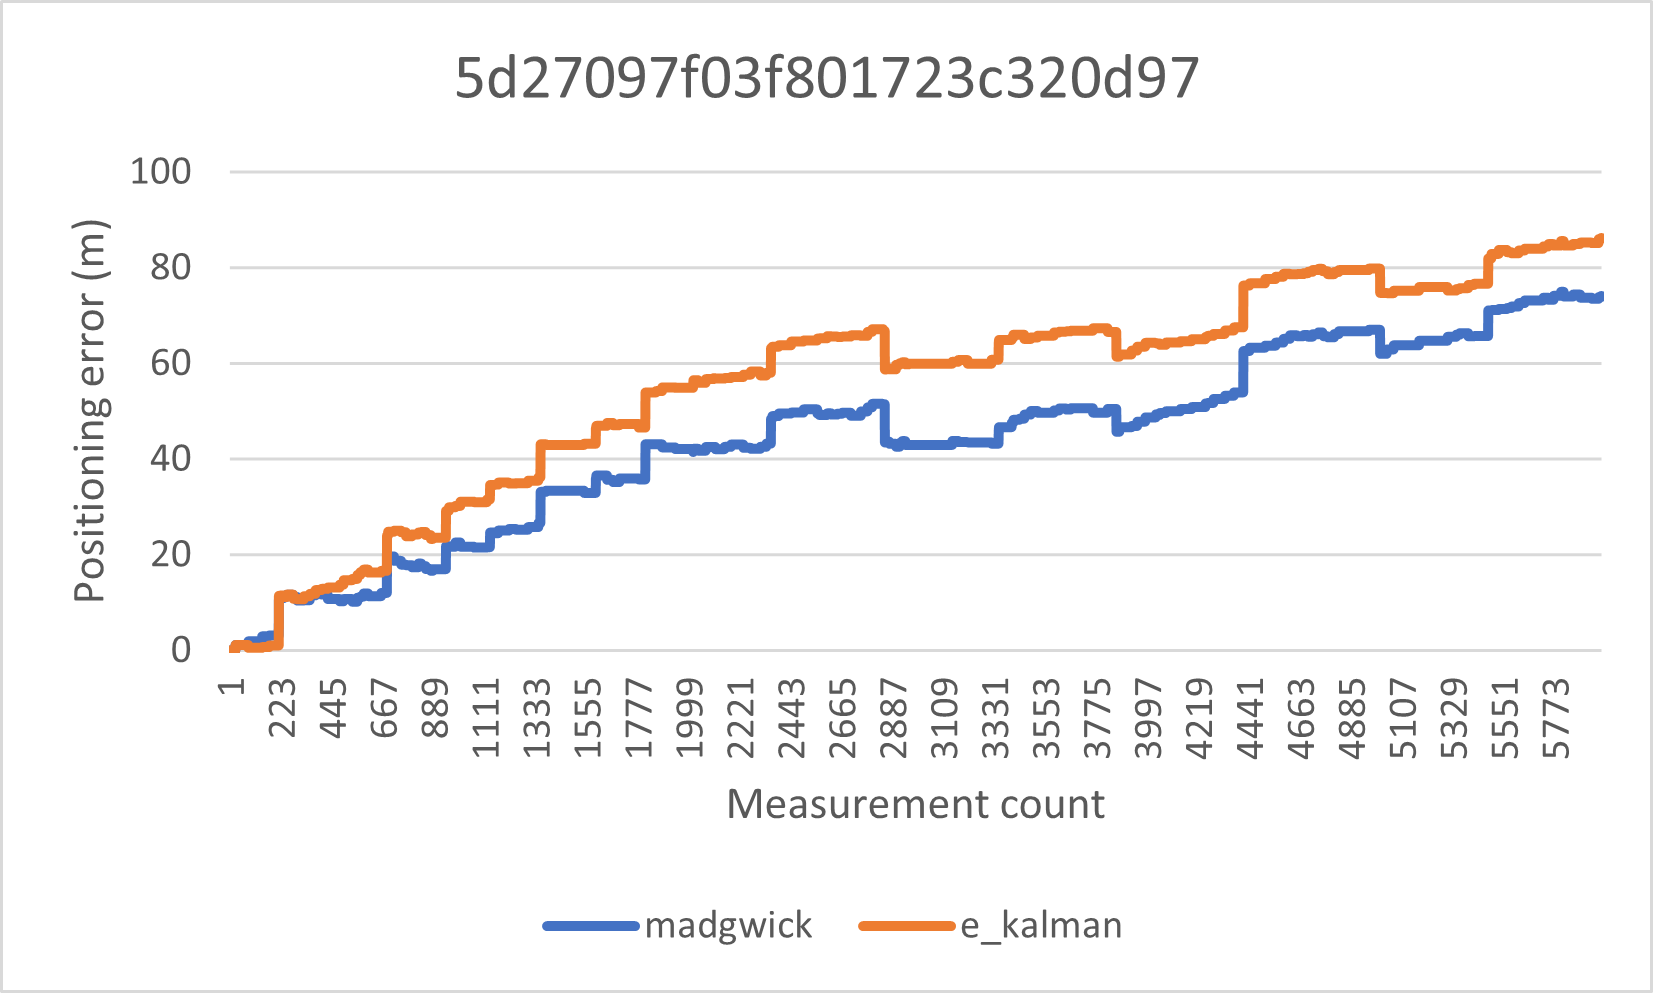
\includegraphics{Images/Experiments/pdr/pdr10.png}}
  \hfill
  \subfigure[]{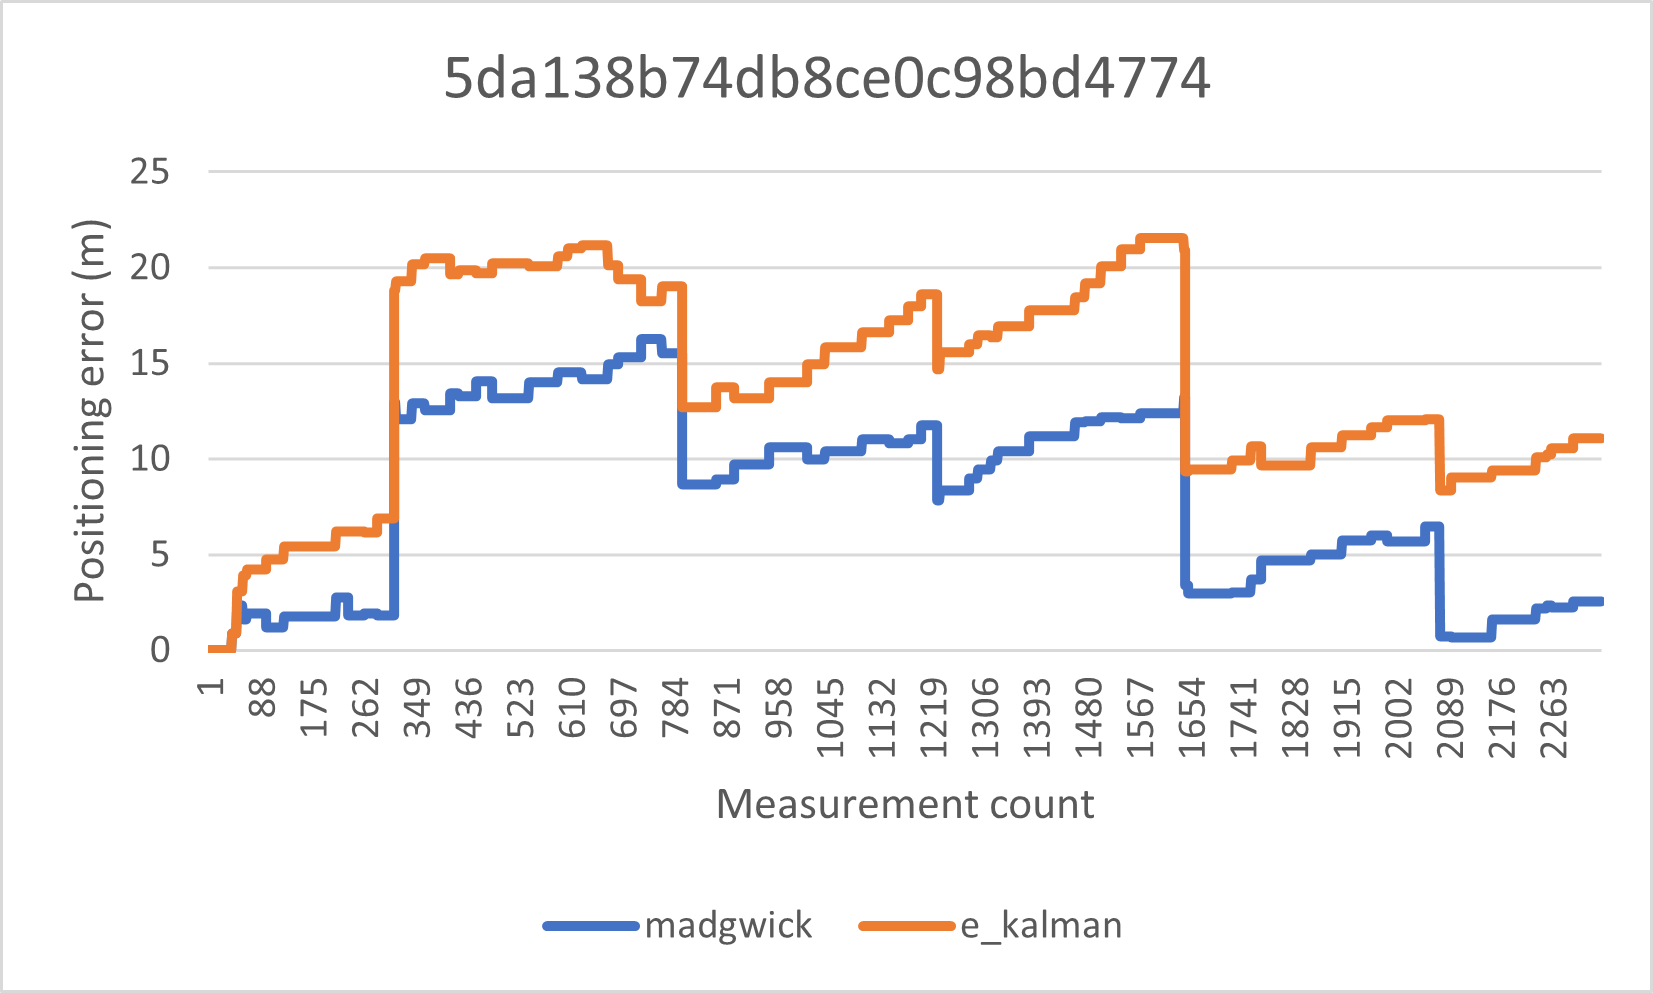
\includegraphics{Images/Experiments/pdr/pdr12.png}}
  \hfill
  \subfigure[]{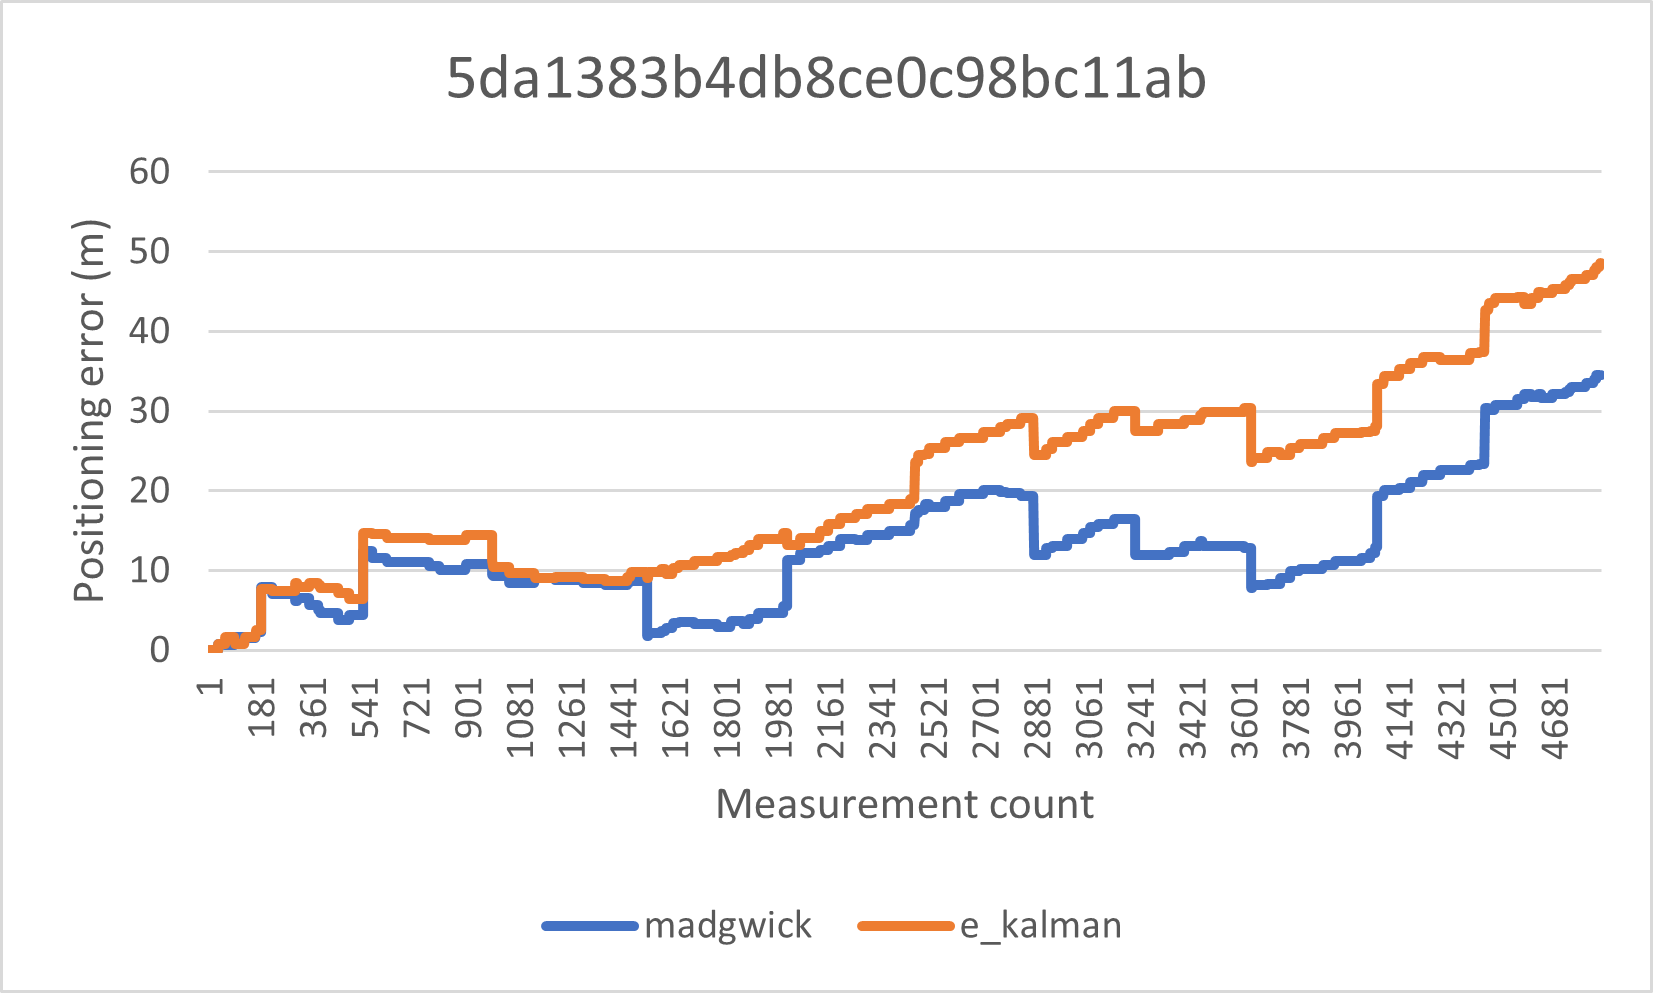
\includegraphics{Images/Experiments/pdr/pdr15.png}}
  \hfill
  \caption{\gls{pdr} performance using Madgwick Filter and Extended Kalman Filter for heading estimation.}
  \label{fig:pdr_performance}
\end{figure}

Furthermore, we have analysed the timestamps between the measurements. The longer the \gls{pdr} algorithm has to wait till next measurement, the more likely the position estimation is to be inaccurate. On \textbf{\autoref{fig:pdr_boxplot}} is seen a diagram that depicts the minimum, maximum and median variance in measurement timestamps.

\begin{figure}[H]
    \centering
    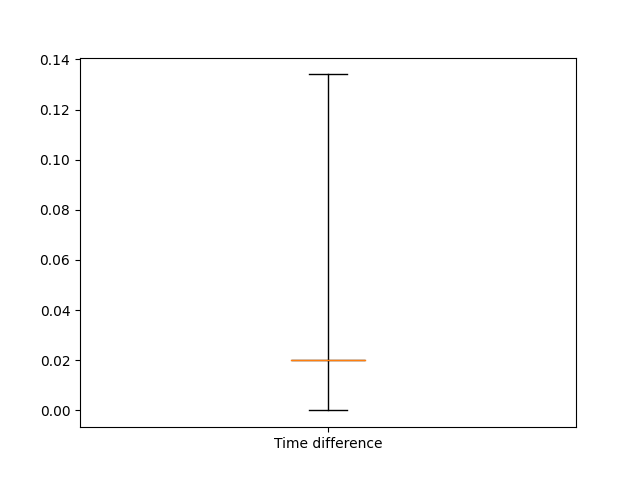
\includegraphics[scale = 0.55]{Images/Experiments/pdr/boxplot.png}
    \caption{Variance in measurement timestamps in seconds. The lowest line is the minimum timestamp difference, the middle line is the median and the highest line is the maximum.}
    \label{fig:pdr_boxplot}
\end{figure}

As seen on \textbf{\autoref{fig:pdr_boxplot}}, there is quite a difference from the median to the maximum measurement timestamp difference. The middle line consists of three lines; the median, 1st quartile and 3rd quartile. Because these three lines are so close to each other, it means that only a few of the measurement timestamps differ more than 0.02 from the previous measurement timestamp. These few measurement timestamps that differ more than 0.02 may be the reason to some of the major wrong heading estimations, since the heading estimation is based on receiving data with a given frequency. Therefore, these few measurement timestamps will temporarily decrease the expected frequency.

As seen on \textbf{\autoref{fig:pdr_cdf}}, it is clear that the Madgwick Filter implementation outperforms the Extended Kalman Filter implementation by their \gls{cdf}, since it can be seen in \textbf{\autoref{fig:pdr_cdf}(b)} that positioning errors using Extended Kalman Filter reach higher position error values with 565.02 meters for 100\% of the data compared to using Madgwick Filter with a positioning error of 400.40 meters for 100 \% of the data, seen in \textbf{\autoref{fig:pdr_cdf}(a)}. Furthermore, the positive slope of \gls{cdf} decreases at positioning error around 50 meters for \textbf{\autoref{fig:pdr_cdf}(a)}, whereas this does not happen until at around 100 meters for \textbf{\autoref{fig:pdr_cdf}(b)}. This generally means that the Extended Kalman Filter implementation outputs position estimations that are further off the ground truth position compared to the Madgwick Filter implementation.

\begin{figure}[H]
\centering
  \SetFigLayout{1}{2}
  \subfigure[]{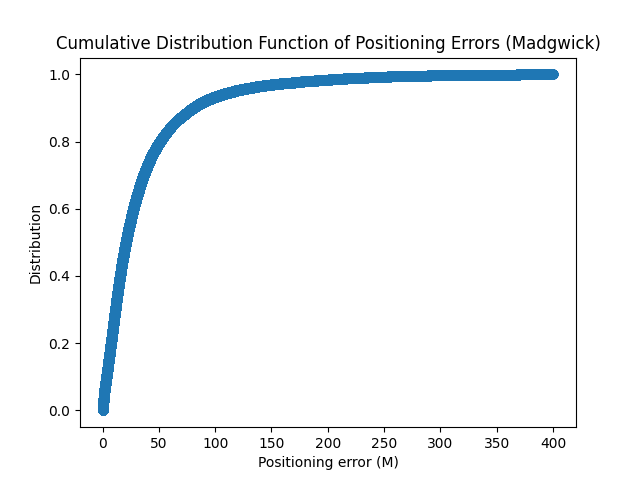
\includegraphics{Images/Experiments/pdr/cdf_madgwick.png}}
  \hfill
  \subfigure[]{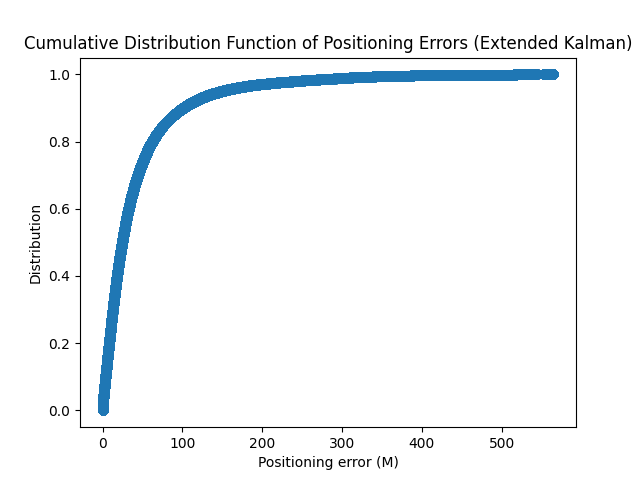
\includegraphics{Images/Experiments/pdr/cdf_kalman.png}}
  \caption{\gls{cdf} for Madgwick Filter implementation (a) and Extended Kalman Filter implementation (b).}
  \label{fig:pdr_cdf}
\end{figure}

Because the \gls{pdr} algorithm performs best using Madgwick Filter, this will be our choice of heading estimation filter for the algorithm.